\documentclass[conference]{IEEEtran}

% Some very useful LaTeX packages include:
% (uncomment the ones you want to load)


% *** MISC UTILITY PACKAGES ***
%
%\usepackage{ifpdf}
% Heiko Oberdiek's ifpdf.sty is very useful if you need conditional
% compilation based on whether the output is pdf or dvi.
% usage:
% \ifpdf
%   % pdf code
% \else
%   % dvi code
% \fi
% The latest version of ifpdf.sty can be obtained from:
% http://www.ctan.org/pkg/ifpdf
% Also, note that IEEEtran.cls V1.7 and later provides a builtin
% \ifCLASSINFOpdf conditional that works the same way.
% When switching from latex to pdflatex and vice-versa, the compiler may
% have to be run twice to clear warning/error messages.

% *** CITATION PACKAGES ***
%
%\usepackage{cite}
% cite.sty was written by Donald Arseneau
% V1.6 and later of IEEEtran pre-defines the format of the cite.sty package
% \cite{} output to follow that of the IEEE. Loading the cite package will
% result in citation numbers being automatically sorted and properly
% "compressed/ranged". e.g., [1], [9], [2], [7], [5], [6] without using
% cite.sty will become [1], [2], [5]--[7], [9] using cite.sty. cite.sty's
% \cite will automatically add leading space, if needed. Use cite.sty's
% noadjust option (cite.sty V3.8 and later) if you want to turn this off
% such as if a citation ever needs to be enclosed in parenthesis.
% cite.sty is already installed on most LaTeX systems. Be sure and use
% version 5.0 (2009-03-20) and later if using hyperref.sty.
% The latest version can be obtained at:
% http://www.ctan.org/pkg/cite
% The documentation is contained in the cite.sty file itself.

% *** GRAPHICS RELATED PACKAGES ***
%
%\ifCLASSINFOpdf
  % \usepackage[pdftex]{graphicx}
  % declare the path(s) where your graphic files are
  % \graphicspath{{../pdf/}{../jpeg/}}
  % and their extensions so you won't have to specify these with
  % every instance of \includegraphics
  % \DeclareGraphicsExtensions{.pdf,.jpeg,.png}
%\else
  % or other class option (dvipsone, dvipdf, if not using dvips). graphicx
  % will default to the driver specified in the system graphics.cfg if no
  % driver is specified.
  % \usepackage[dvips]{graphicx}
  % declare the path(s) where your graphic files are
  % \graphicspath{{../eps/}}
  % and their extensions so you won't have to specify these with
  % every instance of \includegraphics
  % \DeclareGraphicsExtensions{.eps}
%\fi
% graphicx was written by David Carlisle and Sebastian Rahtz. It is
% required if you want graphics, photos, etc. graphicx.sty is already
% installed on most LaTeX systems. The latest version and documentation
% can be obtained at: 
% http://www.ctan.org/pkg/graphicx
% Another good source of documentation is "Using Imported Graphics in
% LaTeX2e" by Keith Reckdahl which can be found at:
% http://www.ctan.org/pkg/epslatex
%
% latex, and pdflatex in dvi mode, support graphics in encapsulated
% postscript (.eps) format. pdflatex in pdf mode supports graphics
% in .pdf, .jpeg, .png and .mps (metapost) formats. Users should ensure
% that all non-photo figures use a vector format (.eps, .pdf, .mps) and
% not a bitmapped formats (.jpeg, .png). The IEEE frowns on bitmapped formats
% which can result in "jaggedy"/blurry rendering of lines and letters as
% well as large increases in file sizes.
%
% You can find documentation about the pdfTeX application at:
% http://www.tug.org/applications/pdftex
\usepackage{graphicx}

% *** MATH PACKAGES ***
%
\usepackage{latexsym}
\usepackage{amsmath}
% A popular package from the American Mathematical Society that provides
% many useful and powerful commands for dealing with mathematics.
%
% Note that the amsmath package sets \interdisplaylinepenalty to 10000
% thus preventing page breaks from occurring within multiline equations. Use:
%\interdisplaylinepenalty=2500
% after loading amsmath to restore such page breaks as IEEEtran.cls normally
% does. amsmath.sty is already installed on most LaTeX systems. The latest
% version and documentation can be obtained at:
% http://www.ctan.org/pkg/amsmath

% *** SPECIALIZED LIST PACKAGES ***
%
%\usepackage{algorithmic}
% algorithmic.sty was written by Peter Williams and Rogerio Brito.
% This package provides an algorithmic environment fo describing algorithms.
% You can use the algorithmic environment in-text or within a figure
% environment to provide for a floating algorithm. Do NOT use the algorithm
% floating environment provided by algorithm.sty (by the same authors) or
% algorithm2e.sty (by Christophe Fiorio) as the IEEE does not use dedicated
% algorithm float types and packages that provide these will not provide
% correct IEEE style captions. The latest version and documentation of
% algorithmic.sty can be obtained at:
% http://www.ctan.org/pkg/algorithms
% Also of interest may be the (relatively newer and more customizable)
% algorithmicx.sty package by Szasz Janos:
% http://www.ctan.org/pkg/algorithmicx

% *** ALIGNMENT PACKAGES ***
%
%\usepackage{array}
% Frank Mittelbach's and David Carlisle's array.sty patches and improves
% the standard LaTeX2e array and tabular environments to provide better
% appearance and additional user controls. As the default LaTeX2e table
% generation code is lacking to the point of almost being broken with
% respect to the quality of the end results, all users are strongly
% advised to use an enhanced (at the very least that provided by array.sty)
% set of table tools. array.sty is already installed on most systems. The
% latest version and documentation can be obtained at:
% http://www.ctan.org/pkg/array

% IEEEtran contains the IEEEeqnarray family of commands that can be used to
% generate multiline equations as well as matrices, tables, etc., of high
% quality.

% *** SUBFIGURE PACKAGES ***
%\ifCLASSOPTIONcompsoc
%  \usepackage[caption=false,font=normalsize,labelfont=sf,textfont=sf]{subfig}
%\else
%  \usepackage[caption=false,font=footnotesize]{subfig}
%\fi
% subfig.sty, written by Steven Douglas Cochran, is the modern replacement
% for subfigure.sty, the latter of which is no longer maintained and is
% incompatible with some LaTeX packages including fixltx2e. However,
% subfig.sty requires and automatically loads Axel Sommerfeldt's caption.sty
% which will override IEEEtran.cls' handling of captions and this will result
% in non-IEEE style figure/table captions. To prevent this problem, be sure
% and invoke subfig.sty's "caption=false" package option (available since
% subfig.sty version 1.3, 2005/06/28) as this is will preserve IEEEtran.cls
% handling of captions.
% Note that the Computer Society format requires a larger sans serif font
% than the serif footnote size font used in traditional IEEE formatting
% and thus the need to invoke different subfig.sty package options depending
% on whether compsoc mode has been enabled.
%
% The latest version and documentation of subfig.sty can be obtained at:
% http://www.ctan.org/pkg/subfig

% *** FLOAT PACKAGES ***
%
%\usepackage{fixltx2e}
% fixltx2e, the successor to the earlier fix2col.sty, was written by
% Frank Mittelbach and David Carlisle. This package corrects a few problems
% in the LaTeX2e kernel, the most notable of which is that in current
% LaTeX2e releases, the ordering of single and double column floats is not
% guaranteed to be preserved. Thus, an unpatched LaTeX2e can allow a
% single column figure to be placed prior to an earlier double column
% figure.
% Be aware that LaTeX2e kernels dated 2015 and later have fixltx2e.sty's
% corrections already built into the system in which case a warning will
% be issued if an attempt is made to load fixltx2e.sty as it is no longer
% needed.
% The latest version and documentation can be found at:
% http://www.ctan.org/pkg/fixltx2e

%\usepackage{stfloats}
% stfloats.sty was written by Sigitas Tolusis. This package gives LaTeX2e
% the ability to do double column floats at the bottom of the page as well
% as the top. (e.g., "\begin{figure*}[!b]" is not normally possible in
% LaTeX2e). It also provides a command:
%\fnbelowfloat
% to enable the placement of footnotes below bottom floats (the standard
% LaTeX2e kernel puts them above bottom floats). This is an invasive package
% which rewrites many portions of the LaTeX2e float routines. It may not work
% with other packages that modify the LaTeX2e float routines. The latest
% version and documentation can be obtained at:
% http://www.ctan.org/pkg/stfloats
% Do not use the stfloats baselinefloat ability as the IEEE does not allow
% \baselineskip to stretch. Authors submitting work to the IEEE should note
% that the IEEE rarely uses double column equations and that authors should try
% to avoid such use. Do not be tempted to use the cuted.sty or midfloat.sty
% packages (also by Sigitas Tolusis) as the IEEE does not format its papers in
% such ways.
% Do not attempt to use stfloats with fixltx2e as they are incompatible.
% Instead, use Morten Hogholm'a dblfloatfix which combines the features
% of both fixltx2e and stfloats:
%
% \usepackage{dblfloatfix}
% The latest version can be found at:
% http://www.ctan.org/pkg/dblfloatfix

% *** PDF, URL AND HYPERLINK PACKAGES ***
%
%\usepackage{url}
% url.sty was written by Donald Arseneau. It provides better support for
% handling and breaking URLs. url.sty is already installed on most LaTeX
% systems. The latest version and documentation can be obtained at:
% http://www.ctan.org/pkg/url
% Basically, \url{my_url_here}.

% *** Do not adjust lengths that control margins, column widths, etc. ***
% *** Do not use packages that alter fonts (such as pslatex).         ***
% There should be no need to do such things with IEEEtran.cls V1.6 and later.
% (Unless specifically asked to do so by the journal or conference you plan
% to submit to, of course. )

% correct bad hyphenation here
%\hyphenation{op-tical net-works semi-conduc-tor}

\newcommand{\adj}[1]{A^{[#1]}}

\begin{document}
\title{Small-World Behavior in Time-Varying Interaction Networks}

% author names and affiliations
% use a multiple column layout for up to three different
% affiliations
\author{\IEEEauthorblockN{William Vining}
  \IEEEauthorblockA{Department of Computer Science\\
    University of New Mexico\\
    Email: wfvining@cs.unm.edu}
}

% conference papers do not typically use \thanks and this command
% is locked out in conference mode. If really needed, such as for
% the acknowledgment of grants, issue a \IEEEoverridecommandlockouts
% after \documentclass

% for over three affiliations, or if they all won't fit within the width
% of the page, use this alternative format:
% 
%\author{\IEEEauthorblockN{Michael Shell\IEEEauthorrefmark{1},
%Homer Simpson\IEEEauthorrefmark{2},
%James Kirk\IEEEauthorrefmark{3}, 
%Montgomery Scott\IEEEauthorrefmark{3} and
%Eldon Tyrell\IEEEauthorrefmark{4}}
%\IEEEauthorblockA{\IEEEauthorrefmark{1}School of Electrical and Computer Engineering\\
%Georgia Institute of Technology,
%Atlanta, Georgia 30332--0250\\ Email: see http://www.michaelshell.org/contact.html}
%\IEEEauthorblockA{\IEEEauthorrefmark{2}Twentieth Century Fox, Springfield, USA\\
%Email: homer@thesimpsons.com}
%\IEEEauthorblockA{\IEEEauthorrefmark{3}Starfleet Academy, San Francisco, California 96678-2391\\
%Telephone: (800) 555--1212, Fax: (888) 555--1212}
%\IEEEauthorblockA{\IEEEauthorrefmark{4}Tyrell Inc., 123 Replicant Street, Los Angeles, California 90210--4321}}

\maketitle

% As a general rule, do not put math, special symbols or citations
% in the abstract
\begin{abstract}
The abstract goes here.
\end{abstract}

% no keywords

% For peer review papers, you can put extra information on the cover
% page as needed:
% \ifCLASSOPTIONpeerreview
% \begin{center} \bfseries EDICS Category: 3-BBND \end{center}
% \fi
%
% For peerreview papers, this IEEEtran command inserts a page break and
% creates the second title. It will be ignored for other modes.
\IEEEpeerreviewmaketitle

\section{Introduction}
\label{sec:intro}
In many natural systems complex behavior emerges as a result of the
interactions of large numbers independent agents. For example in ant
colonies efficient paths to food are discovered by a single ant, and
exploited by the entire colony. The knowledge of the food is passed to
the rest of the ants either through direct interactions, or
stygmergy. As another example, ant colonies modulate the rate at which
they leave the nest to forage based on interactions with returning
foragers~\cite{Pinter2013}. The interactions between agents (in this
example ants) can be represented as a network where vertices are
individual agents and edges are placed between agents that interact,
or are in close enough proximity that they could interact. Such
networks change on very rapid time-scales and at any given moment are
extremely sparse. This paper investigates what role different types of
random movement and different densities of agents can play in the
structure of these networks. We establish what types of movement are
most 

Static or slow changing networks are well studied and exhibit many
interesting phenomena. Notably the small-world phenomenon described by
Watts and Storgatz~\cite{Watts1998} leads to short path lengths,
despite the highly regular structure of the network. Because they are
amenable to mathematical analysis networks provide an excellent model
for studying phenomena such as interactions. Much of the research
investigating networks is focused on the case of static or slowly
growing networks (for example the model of preferential attachment of
Barab\'asi and Albert~\cite{Barabasi1999}). Many complex systems,
however, are best described by networks where edges are frequently
being added and removed. This is the case for the example of ants
given above, or even emerging technologies such as the internet of
things. Recently some effort has been made to generalize the
mathematical methods for analyzing static networks to apply them to
dynamic networks. Of particular interest are measures of
communicability described by Grindrod et al.~\cite{Grindrod2011} and
the generalization of small-world behavior described
by~\cite{Tang2010}.

This paper applies these methods to the analysis of dynamic networks
representing interactions between agents moving in a finite space. We
aim to determine how the movement patterns impact the properties of
the interaction network particularly in terms of how effectively
agents can communicate. An improved understanding of these properties
may be useful in the design of algorithms for robot swarms by
characterizing the trade offs between movement strategies and the
effectiveness with which information can be disseminated among members
of the swarm. The following section presents relevant background on
time-varying graphs and the mathematics used for the analysis in this
paper. Following that we will present the experiments and results
which show that particular movement types such as a correlated random
walk have limited impact on communicability while other movement types
can have a dramatic impact.

\subsection{Background}
\label{subsec:bg}
The typical representation of a dynamic network is an ordered sequence
of graphs each representing a snapshot of the structure of the network
at a particular point in time. This structure is called a time-varying
graph, an example of such a graph is shown in
figure~\ref{fig:tvg}. This representation inherently coarse-grains the
evolution of the network and can cause important structures to be
masked or other bias to be introduced~\cite{Clauset2007}. Other
researchers have studied dynamic network models in continuous time in
order to address these biases, for example~\cite{Grindrod2014}. For the purposes of
this paper, however, we are concerned only with discrete snapshots,
and assume that the sampling frequency is on roughly the same scale as
the rate at which messages can be exchanged between agents. It is
important to note that in general a snapshot will not be
connected. The only way a message can propagate from one vertex to
another is through time, which can lead to an inherent asymmetry in
paths: the existence of a path from $a \leadsto b$ does not imply that
a path $b \leadsto a$ exists, even in the case where snapshots are not
directed~\cite{Tang2010}.

\begin{figure}
  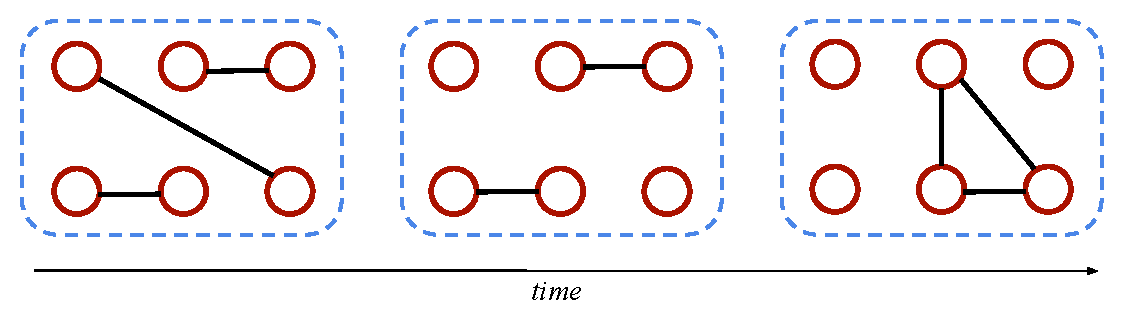
\includegraphics[width=\columnwidth]{tvg}
  \caption{A time varying graph evolving over three time-steps.}
  \label{fig:tvg}
\end{figure}

Tang et al~\cite{Tang2010} described a generalization of small-world
behavior to dynamic networks. They used a metric developed by Clauset
and Eagle~\cite{Clauset2007} to quantify the similarity of consecutive
snapshots. The measure, called the \emph{temporal correlation
  coefficient} (TCC), is given by
\begin{equation}
  C = \frac{1}{N}\sum_{i = 1}^N C_i, C_i = \frac{1}{T-1}\sum_{t=1}^{T-1} \frac{\sum_j A_{ij}^{[t]}A_{ij}^{[t+1]}}{\sqrt{(\sum_j A_{ij}^{[t]})(\sum_j A_{ij}^{[t+1]})}}.
  \label{eq:tcc}
\end{equation}
Where $\adj{t}$ is the adjacency matrix of the snapshot at time $t$,
$T$ is the number of snapshots, and $N$ is the number of agents. If
one of the rows in $\adj{t}$ or $\adj{t+1}$ is entirely 0s then $C_i$
is defined to be 1. This equation has the property that if every
snapshot is identical then $C = 1$. The authors use a generalized
version of breadth-first search to compute the all-pairs minimum path
length. The generalized algorithm builds a frontier of discovered
nodes by adding all adjacent, undiscovered, nodes in the current
snapshot $\adj{t}$ to the frontier then moves to the next snapshot
$\adj{t+1}$. This enforces the condition that only one edge can be
traversed per time-step (we can allow multiple edges by inserting
repeated copies of each snapshot). The temporal distance $d_{ij}$
between $i$ and $j$ is $t$ if $j$ is discovered in snapshot $\adj{t}$
when the search begins at $i$ in snapshot $\adj{1}$. Note that there
are implicit self-loops in this model. A temporal path may consist of
staying at the same node for many time-steps before the target node is
discovered. The \emph{characteristic temporal path length} (CTPL) is
then defined as
\begin{equation}
  L = \frac{1}{N-1} \sum_{ij}d_{ij}.
  \label{eq:ctpl}
\end{equation}
In the case
where no path from $i$ to $j$ exists, $d_{ij} = \infty$ and we exclude
that path from the average. Using these two metrics Tang et al define
small world behavior to be when a time-varying graph exhibits high
temporal correlation ($C$) and low characteristic temporal path
lengths ($L$).

In addition to the equations above, Tang et al~\cite{Tang2010}
presented a model for building interaction networks that we build on
here. In the Tang et al model each agent moves with constant velocity
in a fixed 100 by 100 meter space. With probability $p_j$ the agent is
``teleported'' to another location in that space at each time-step. At
each second a snapshot is created with an edge between any agents that
are within 5 meters of each other (this is called the
\emph{communication radius}). We expand on this model by changing the
motion of the agents, as described in section~\ref{sec:methods}, to
simulate a correlated random walk, Brownian motion and a L\'evy
flight.

We are not just interested in the structure of the network, but also
in how effectively agents can communicate over that structure. In the
static network setting a common measure of this is the centrality of
each node. In particular we are interested in the Katz
centrality~\cite{Newman2010} which measures the number of walks
between each pair of node. Long walks are weighted less heavily than
short walks corresponding to the idea that a message is likely to
degrade the more times it is transmitted. Grindrod et
al~\cite{Grindrod2011} generalized Katz centrality to apply it to
walks in time varying graphs. This equation measures walks that use
edges in a time-ordered sequence of adjacency matrices. Grindrod et
al. note that, because it is non-commutative, measures based on matrix
multiplications are well suited to analyzing time-varying graphs since
they implicitly preserve the ``arrow of time.'' The generalized Katz
centrality is given the following equation
\begin{equation}
  Q = \prod_{t = 1}^T(I - \alpha \adj{t})^{-1}.
  \label{eq:q}
\end{equation}
$Q$ is referred to as the \emph{communicability matrix} and its
row-sums and column-sums tell us how effectively each node can
broadcast or receive a message respectively. The walks counted by $Q$
include those which use arbitrarily many edges from each snapshot
which is not what we are interested in for the purposes of this
paper. The authors present another matrix multiplication
(equation~\ref{eq:qoh}) that computes the same metric, but limits the
number of edges that can be traversed in each snapshot to 1.
\begin{equation}
  Q^{onehop} = \prod_{t = 1}^T(I + \alpha \adj{t})
  \label{eq:qoh}
\end{equation}

The remainder of this paper describes the extensions to the
agent-based model of Tang et al~\cite{Tang2010} and the evaluation of
the resulting interaction networks. We then discuss the implications
of these results for the design of distributed algorithms for robotic
swarms.

\section{Methods}
\label{sec:methods}

The interaction networks that are analyzed below were generated by a
model of $N$ agents moving in a 100 meter square ``arena.'' The walls
of the arena are impenetrable, agents that hit a wall reflect off of
it. Agents are modeled as particles placed in a rectangle at the
center of the arena with 1m separating each agent. The initial heading
of each agent is directly away from the center of the arena and the
initial velocity is 1 m/s. There are no collisions between agents, if
two agents happen to occupy the same exact location, they pass through
each other. At each second a snapshot $\adj{t}$ is generated where
\begin{equation}
  \adj{t}_{ij} = \begin{cases} 1 & d(i, j) < r \\ 0 & \text{otherwise} \end{cases}
  \label{eq:snapshot}
\end{equation}
where $d(i,j)$ is the distance between agent $i$ and agent $j$ and $r$
is the communication radius (for this paper $r = 5 m$). Thus snapshot
$\adj{t}$ represents which agents \emph{can} exchange a message at
time $t$ but not which agents actively communicate. The model is run
for 1000 seconds before snapshots are recorded to allow agents to
disperse and reach an equilibrium state. Without discarding the
initial time-steps, every interaction network is biased towards very
short CTPL.

Three distinct types of movement were implemented for agents in the
model (summarized in table~\ref{tab:strat}). In two movement
strategies, the correlated random walk (CRW) and the teleportation
model from~\cite{Tang2010} (described in section~\ref{subsec:bg}),
agent speed remained constant. Agents using the CRW strategy moved
with a constant speed of 1 m/s and once per second selected a new
heading from a normal distribution $\mathcal{N}(0,
\sigma)$. Experiments were conducted with $\sigma = \pi/4, \pi/2,
3\pi/4,$ and $\pi$. We also implemented a L\'evy flight where, once
per second, agents select a new heading uniformly at random from the
range $[0,2\pi]$ and additionally select a new speed in the range $[1,
  r]$ such that step sizes have a power law distribution with smaller
sizes more common than larger step sizes. Specifically, the
probability of a step size $x$ is given by $\lambda(x) \simeq
x^{(-1-\alpha)}$ where $0 < \alpha \le 2$~\cite{Chechkin2008}.

\begin{table}
  \begin{center}
  \begin{tabular}{l l l}
    Strategy & speed    & heading \\\hline
    Teleport & 1 m/s & reflection only \\
    CRW      & 1 m/s & $\mathcal{N}(0, \sigma)$ \\
    L\'evy   & Powerlaw(1,5) & $\mathcal{U}(0,2\pi)$
  \end{tabular}
  \end{center}
  \caption{Summary of movement strategies}
  \label{tab:strat}
\end{table}

Each movement strategy was used to generate interaction networks for
4, 8, 16, 32, 128, 256, and 512 agents (the L\'evy flight strategy was
only evaluated up to 128 agents due to time constraints). For each
network the CTPL, TCC, and $Q$ were calculated. The results of these
experiments are presented in the following section.

\section{Results}
\label{sec:results}

The first experiment replicated the work of Tang et al~\cite{Tang2010}
to confirm that the model was implemented correctly. We evaluated the
teleportation model for values of $p_j$ from 0 to 1. The small world
behavior, where the average temporal path length is small and the
temporal correlation is high, can be observed in figure~\ref{fig:swb}.
\begin{figure}
  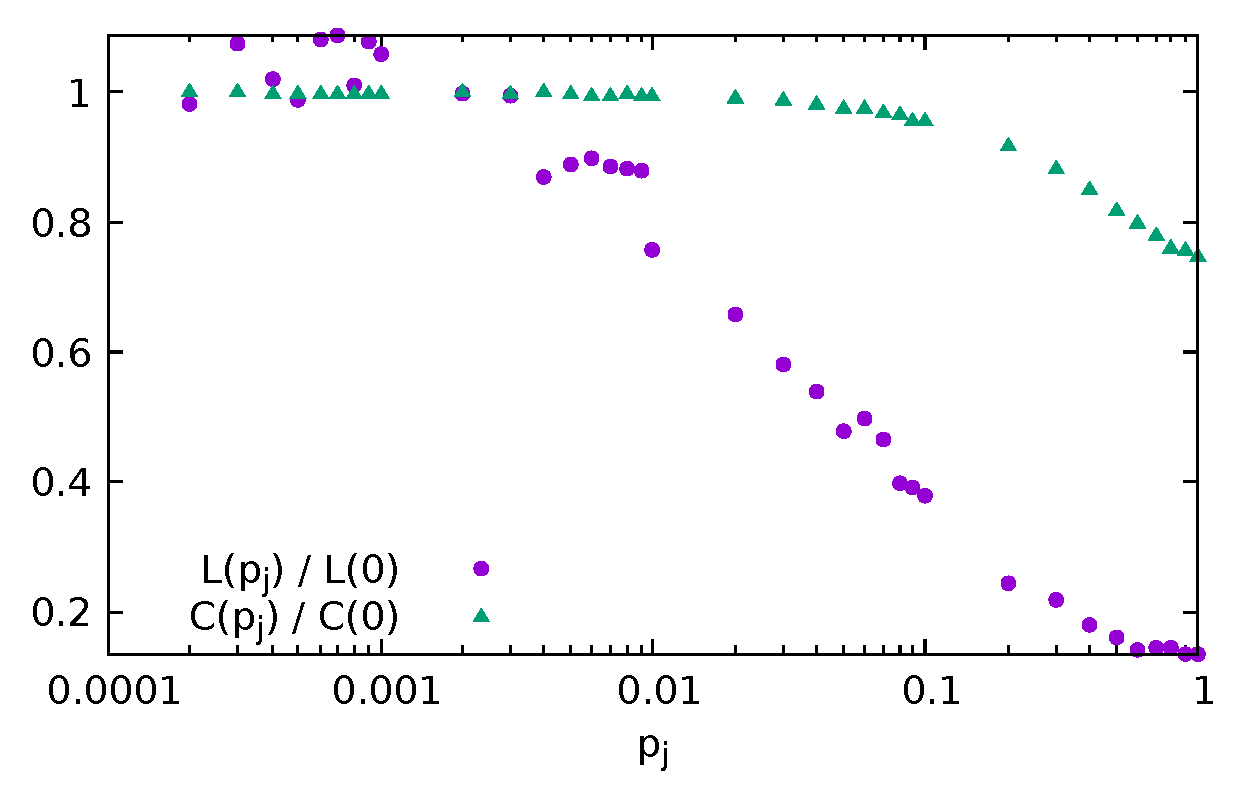
\includegraphics[width=\columnwidth]{teleport-swb.pdf}
  \caption{Small world behavior in the teleportation model for 100
    agents. $L(x)$ and $C(x)$ are the CTPL and TCC respectively for
    the network when $p_j = x$. This does not exactly reproduce the
    results of Tang et al, likely due to differences in the initial
    positions and velocities of the agents.}
  \label{fig:swb}
\end{figure}
The teleportation model was also evaluated for different numbers of
agents. The results are shown in figure~\ref{fig:teleport-scale}. We
observe that as the number of agents increases so does the CTPL.
\begin{figure}
  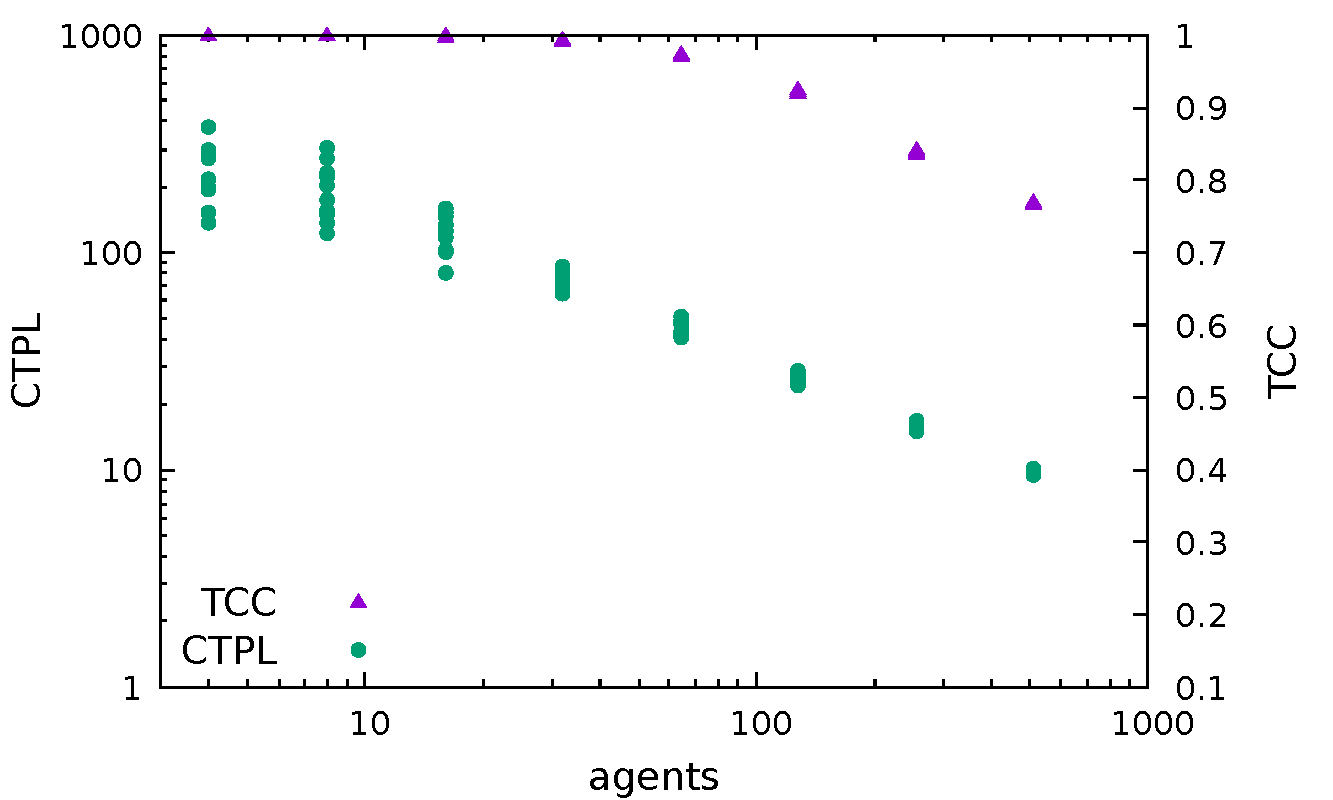
\includegraphics[width=\columnwidth]{teleport-scale.pdf}
  \caption{CTPL for interaction networks produced by the teleportation
    model with 4 to 512 agents}
  \label{fig:teleport-scale}
\end{figure}

\begin{figure}
  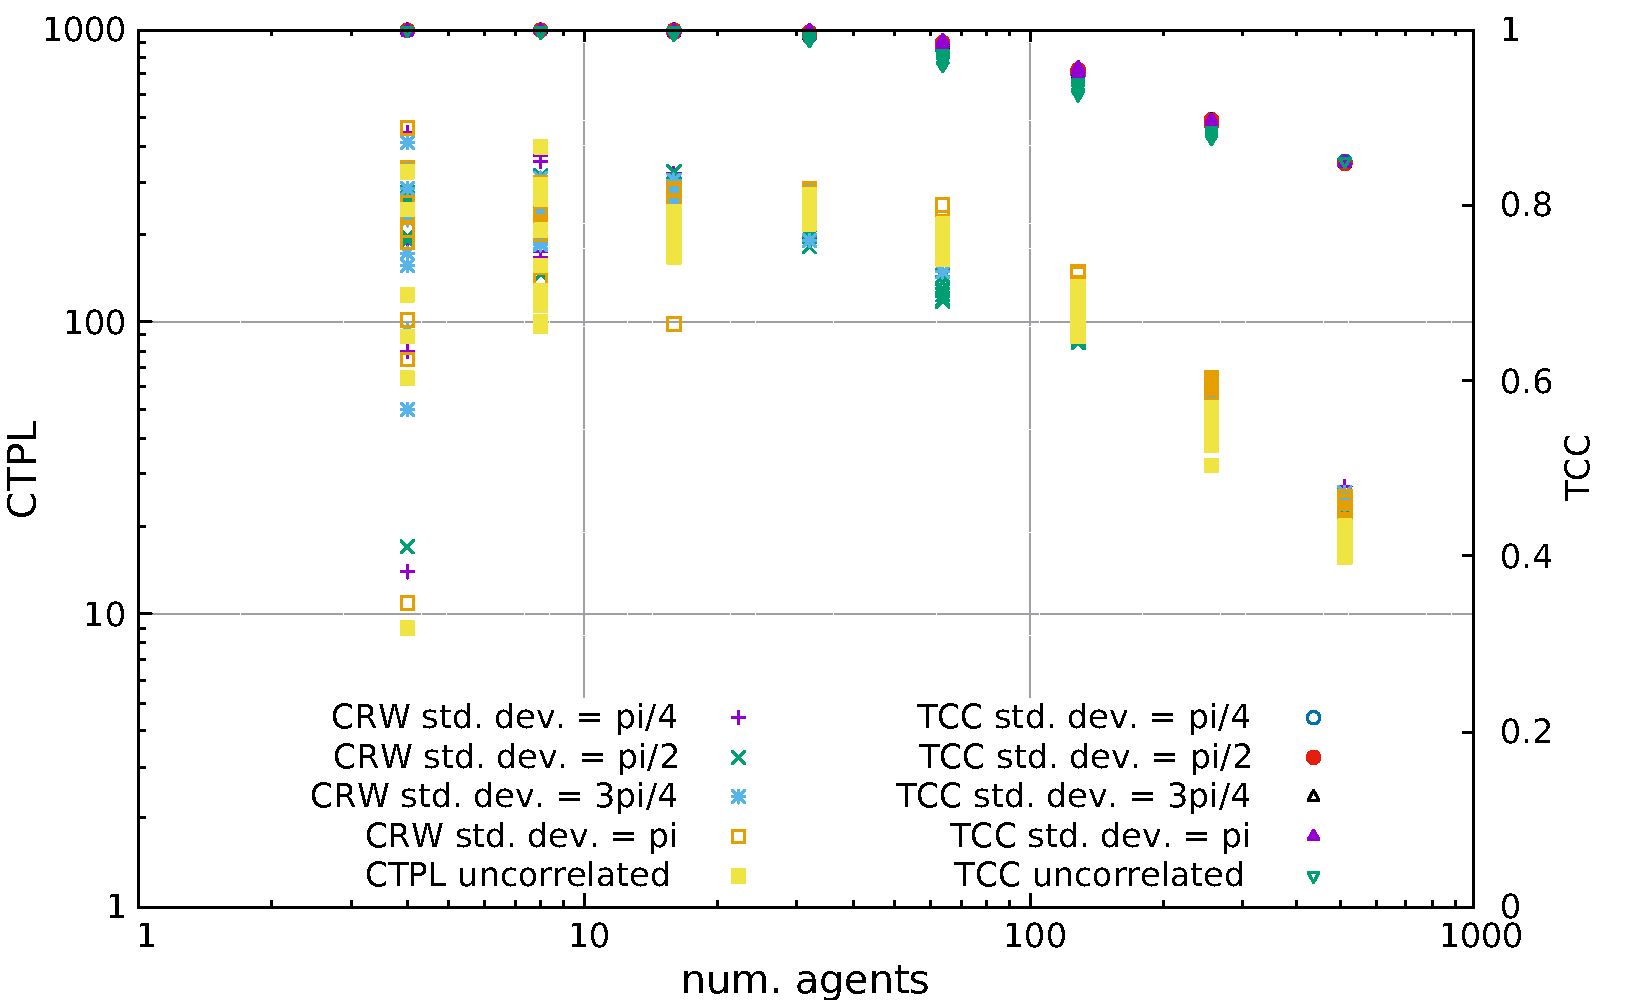
\includegraphics[width=\columnwidth]{correlated-scaling.pdf}
  \caption{Characteristic temporal path length for agents moving with
    a correlated random walk. Agents turn an angle $\theta$ at each
    time-step where $\theta \sim \mathcal{N}(0,\sigma)$, $\sigma$
    ranges from $\pi/4$ to $\pi$ resulting in more or less correlated
    walks respectively. An uncorrelated walk, where $\theta$ is
    unformly distributed in the range $[0, 2\pi]$ is also
    included. CTPL is insensitive to changes in $\sigma$, indicating
    that a correlated walk is equivalent to a simple random walk with
    respect to the average amount of time it takes for a message to
    reach some agent.}
  \label{fig:crw-scale}
\end{figure}

\section{Conclusion}

% An example of a floating figure using the graphicx package.
% Note that \label must occur AFTER (or within) \caption.
% For figures, \caption should occur after the \includegraphics.
% Note that IEEEtran v1.7 and later has special internal code that
% is designed to preserve the operation of \label within \caption
% even when the captionsoff option is in effect. However, because
% of issues like this, it may be the safest practice to put all your
% \label just after \caption rather than within \caption{}.
%
% Reminder: the "draftcls" or "draftclsnofoot", not "draft", class
% option should be used if it is desired that the figures are to be
% displayed while in draft mode.
%
%\begin{figure}[!t]
%\centering
%\includegraphics[width=2.5in]{myfigure}
% where an .eps filename suffix will be assumed under latex, 
% and a .pdf suffix will be assumed for pdflatex; or what has been declared
% via \DeclareGraphicsExtensions.
%\caption{Simulation results for the network.}
%\label{fig_sim}
%\end{figure}

% Note that the IEEE typically puts floats only at the top, even when this
% results in a large percentage of a column being occupied by floats.


% An example of a double column floating figure using two subfigures.
% (The subfig.sty package must be loaded for this to work.)
% The subfigure \label commands are set within each subfloat command,
% and the \label for the overall figure must come after \caption.
% \hfil is used as a separator to get equal spacing.
% Watch out that the combined width of all the subfigures on a 
% line do not exceed the text width or a line break will occur.
%
%\begin{figure*}[!t]
%\centering
%\subfloat[Case I]{\includegraphics[width=2.5in]{box}%
%\label{fig_first_case}}
%\hfil
%\subfloat[Case II]{\includegraphics[width=2.5in]{box}%
%\label{fig_second_case}}
%\caption{Simulation results for the network.}
%\label{fig_sim}
%\end{figure*}
%
% Note that often IEEE papers with subfigures do not employ subfigure
% captions (using the optional argument to \subfloat[]), but instead will
% reference/describe all of them (a), (b), etc., within the main caption.
% Be aware that for subfig.sty to generate the (a), (b), etc., subfigure
% labels, the optional argument to \subfloat must be present. If a
% subcaption is not desired, just leave its contents blank,
% e.g., \subfloat[].


% An example of a floating table. Note that, for IEEE style tables, the
% \caption command should come BEFORE the table and, given that table
% captions serve much like titles, are usually capitalized except for words
% such as a, an, and, as, at, but, by, for, in, nor, of, on, or, the, to
% and up, which are usually not capitalized unless they are the first or
% last word of the caption. Table text will default to \footnotesize as
% the IEEE normally uses this smaller font for tables.
% The \label must come after \caption as always.
%
%\begin{table}[!t]
%% increase table row spacing, adjust to taste
%\renewcommand{\arraystretch}{1.3}
% if using array.sty, it might be a good idea to tweak the value of
% \extrarowheight as needed to properly center the text within the cells
%\caption{An Example of a Table}
%\label{table_example}
%\centering
%% Some packages, such as MDW tools, offer better commands for making tables
%% than the plain LaTeX2e tabular which is used here.
%\begin{tabular}{|c||c|}
%\hline
%One & Two\\
%\hline
%Three & Four\\
%\hline
%\end{tabular}
%\end{table}


% Note that the IEEE does not put floats in the very first column
% - or typically anywhere on the first page for that matter. Also,
% in-text middle ("here") positioning is typically not used, but it
% is allowed and encouraged for Computer Society conferences (but
% not Computer Society journals). Most IEEE journals/conferences use
% top floats exclusively. 
% Note that, LaTeX2e, unlike IEEE journals/conferences, places
% footnotes above bottom floats. This can be corrected via the
% \fnbelowfloat command of the stfloats package.

% conference papers do not normally have an appendix


% use section* for acknowledgment
\section*{Author Contributions}
WV conceived of and executed the research. WV wrote the paper.

% trigger a \newpage just before the given reference
% number - used to balance the columns on the last page
% adjust value as needed - may need to be readjusted if
% the document is modified later
%\IEEEtriggeratref{8}
% The "triggered" command can be changed if desired:
%\IEEEtriggercmd{\enlargethispage{-5in}}

% references section

% can use a bibliography generated by BibTeX as a .bbl file
% BibTeX documentation can be easily obtained at:
% http://mirror.ctan.org/biblio/bibtex/contrib/doc/
% The IEEEtran BibTeX style support page is at:
% http://www.michaelshell.org/tex/ieeetran/bibtex/
\bibliographystyle{IEEEtran}
% argument is your BibTeX string definitions and bibliography database(s)
\bibliography{tvg-smallworld.bib}

% that's all folks
\end{document}


